\lecture{24}{27. November 2025}{Plane stress transformation}

\section{Stress and Strain Transformation}

\subsection{Plane-Stress Transformation}
The general stress state at a point is characterized by six normal and shear stress components as depicted on \Cref{fig:f24_1}a.
This state of stress is, however, not often encountered in actuality.
Instead, most loadings are coplanar and can be analyzed in a \textit{single plane}.
When this is the case, the material is said to be subject to \textit{plane stress}.

\begin{figure} [ht]
  \centering
  
\includegraphics[width=0.5\linewidth]{./figures/f24_1.png}
  \caption{State of stress at a general point.}
  \label{fig:f24_1}
\end{figure}

The general state of plane stress at a point is shown on \Cref{fig:f24_1}b.
This is represented by a combination of two normal stress components, $\sigma_x$, $\sigma_y$, and one shear stress component $\tau_{xy}$, which act on only four faces of the element as shown on \Cref{fig:f24_2}a.
It is worth realizing, that this state of stress is produced on an element having a different orientation $\theta$ as in \Cref{fig:f24_2}b, then it will be subjected to three different stress components, $\sigma_{x'}$, $\sigma_{y'}$, and $\tau_{x'y'}$, measured relative to the $x'$, $y'$ axes. 

\begin{figure} [ht]
  \centering
  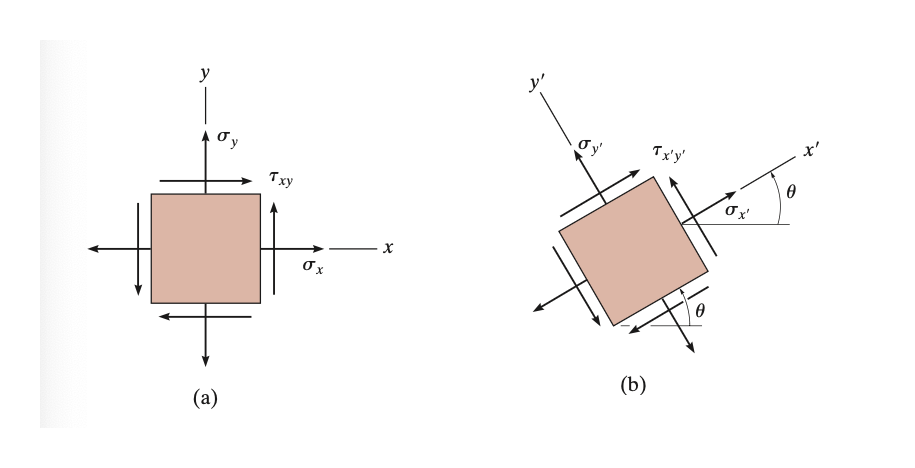
\includegraphics[width=0.5\linewidth]{./figures/f24_2.png}
  \caption{General state of plane stress.}
  \label{fig:f24_2}
\end{figure}

\subsection{General Equations of Plane Stress Transformation}
The method of transforming the normal and shear stress components from the $x,y$ to the $x',y'$ axes, can be developed in a general manner and expressed as a set of stress transformation equations.

\subsubsection{Sign Convention}
As shown on \Cref{fig:f24_5}a, the $+x$ and $+x'$ axes are used to define the outward normal on the right face of the element, so that $\sigma_x$ and $\sigma_{x'}$ are positive, when they act in the positive directions of the $x$ and $x'$ directions, and $\tau_{xy}$ and $\tau_{x'y'}$ are positive when they act in the positive $y$ and $y'$ directions.

\begin{figure} [ht]
  \centering
  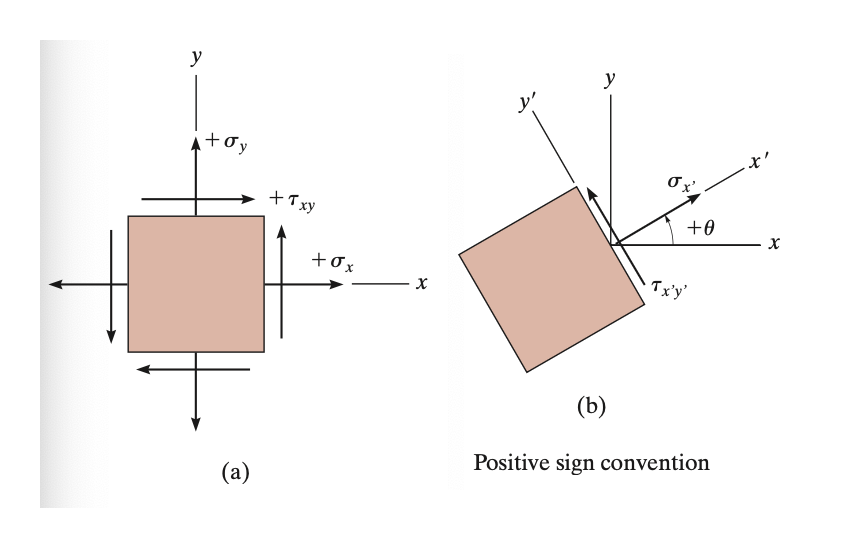
\includegraphics[width=0.8\linewidth]{./figures/f24_5.png}
  \caption{Sign Convention definition}
  \label{fig:f24_5}
\end{figure}

The orientation of the face upon which the normal and shear stress components are to be determined will be defined by the angle $\theta$ which is measured from the $+x$ to the $+x'$ axis, as shown on \Cref{fig:f24_5}b.
This angle is positive following the right hand rule.

\subsubsection{Normal and Shear Stress Components}
The element on \Cref{fig:f24_6}a is sectioned along the inclined plane and the segment shown on \Cref{fig:f24_6}b is isolated.
Assuming the sectioned area is $\Delta A$ then the horizontal and vertical faces of the segment have an area of $\Delta A \sin \theta$ and $\Delta A \cos \theta$, respectively.

\begin{figure} [ht]
  \centering
  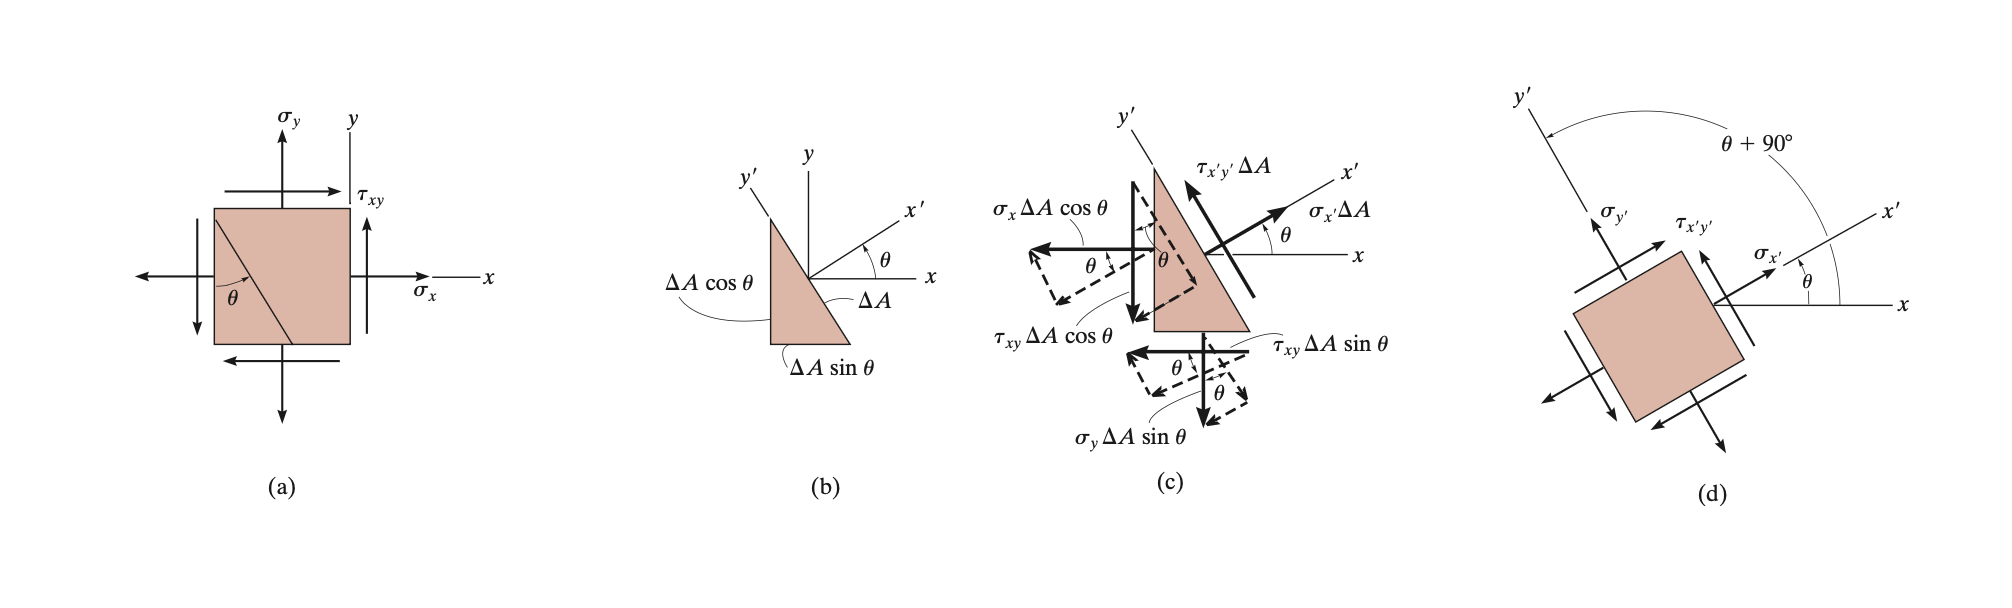
\includegraphics[width=0.8\linewidth]{./figures/f24_6.png}
  \caption{Sectioned element}
  \label{fig:f24_6}
\end{figure}

The resulting free-body diagram is shown on \Cref{fig:f24_6}c.
Using the equations of equilibrium along the $x'$ and $y'$ axes, we can obtain a direct solution for $\sigma_{x'}$ and $\tau_{x'y'}$ as
\begin{align*}
  \sigma_{x'}\Delta A - \left( \tau_{xy} \Delta A \sin \theta \right) \cos \theta - \left( \sigma_y \Delta A \sin \theta \right) \sin \theta - \left( \tau_{xy} \Delta A \cos \theta \right) \sin \theta - \left( \sigma_x \Delta A \cos \theta \right) \cos \theta &= 0 \\
  \sigma_x \cos^2 \theta + \sigma_y \sin^2 \theta + \tau_{xy} \left( 2 \sin \theta \cos \theta\right) &= \sigma_{x'} \\
  \tau_{x'y'} \Delta A + \left( \tau_{xy} \Delta A \sin \theta \right) \sin \theta - \left( \sigma_y \Delta A \sin \theta \right) \cos \theta - \left( \tau_{xy} \Delta A \cos \theta \right) \cos \theta + \left( \sigma_x \Delta A \cos \theta \right) \sin \theta &= 0 \\
  \left( \sigma_y - \sigma_x \right) \sin \theta \cos \theta + \tau_{xy} \left( \cos^2\theta - \sin^2 \theta \right) &= \tau_{x'y'}
.\end{align*}
These two equations can be simplified as:
\begin{align*}
  \sigma_{x'} &= \frac{\sigma_x + \sigma_y}{2} + \frac{\sigma_x - \sigma_y}{2} \cos 2\theta + \tau_{xy} \sin 2\theta \\
  \tau_{x'y'} &= - \frac{\sigma_x - \sigma_y}{2} \sin 2 \theta + \tau_{xy} \cos 2\theta
.\end{align*}

\subsection{Principal Stresses and Maximum In-Plane Shear Stress}
Since $\sigma_x$, $\sigma_y$, and $\tau_{xy}$ are all constant, then the magnitudes of $\sigma_{x'}$ and $\tau_{x'y'}$ only depend on the angle of inclination $\theta$ of the planes of which these stresses act.

\subsubsection{In-Plane Principal Stresses}
To determine the maximum and minimum normal stress, we differentiate the formula for normal stress with respect to $\theta$ and set the result equal to zero.
Solving for $\theta = \theta_p$, which gives the planes of maximum and minimum normal stress yields:
\begin{equation*}
  \tan 2\theta_p = \frac{\tau_{xy}}{\frac{ \sigma_x - \sigma_y}{2}}
.\end{equation*}

To obtain the maximum and minimum normal stress we must then substitute the found angles into the formula for the normal stress.
After substituting and simplifying, the maximum and minimum stresses are:
\begin{equation*}
  \sigma_{1,2} = \frac{\sigma_x + \sigma_y}{2} + \sqrt{\left( \frac{\sigma_x - \sigma_y}{2} \right)^2 + \tau_{xy}^2}
.\end{equation*}
These two values, with $\sigma_1 \geq \sigma_2$ are called the in-plane principal stresses and the planes on which they act are called the principal planes of stress.
No shear-stress acts on the principal planes.


\subsubsection{Maximum In-Plane Shear Stress}
The orientation of the element subjected to maximum shear stress can be determined by taking the derivative of the formula for shear stress with respect to $\theta$ and setting the result equal to zero, yielding:
\begin{equation*}
  \tan 2 \theta_s = \frac{- \frac{\sigma_x - \sigma_y}{2}}{\tau_{xy}}
.\end{equation*}
An element subjected to maximum shear stress will be oriented \ang{45} from the position of an element subjected to the principal stress.

The maximum shear stress can be found as:
\begin{equation*}
  \tau_{\text{max in-plane}} = \pm \sqrt{\left( \frac{\sigma_x - \sigma_y}{2} \right)^2 + \tau_{xy}^2}
.\end{equation*}

The average normal stress on the planes of maximum in-plane shear stress is
\begin{equation*}
  \sigma_{\mathrm{avg}} = \frac{\sigma_x + \sigma_y}{2}
.\end{equation*}

